
%%%%%%%%%%%%%%%%%%%%%%%%%%%%%%%%%%%%%%%%%%%%%%%%%%%%%%%%%%%%%%%%%%%%%%%%
\chapter{Background}
\label{chap:background}
%%%%%%%%%%%%%%%%%%%%%%%%%%%%%%%%%%%%%%%%%%%%%%%%%%%%%%%%%%%%%%%%%%%%%%%%

The chapter sets the stage for the three typed calculi that we are going to
present in later chapters by reviewing some relevant topics in this thesis. In
\cref{bg:sec:intersection} we start with the traditional formulation of
intersection types, followed by an introduction of the merge operator and the
issue of coherence. We then review the \oname calculus, the first calculus
featuring disjoint intersection types, and briefly discuss how disjointness
achieves coherence. In \cref{sec:ernst} we introduce family polymorphism by
means of presenting \citeauthor{ernst2004expression}'s elegant solution to the expression problem.
Finally in \cref{sec:bg:mixin:trait} we review the concepts of mixins and
traits, their drawbacks and strengths.




\section{Intersection Types}
\label{bg:sec:intersection}


Intersection types in the pure $\lambda$-calculus were developed in the late
1970s by \citet{coppoInter}, and independently by \citet{pottinger1980type}. The
original motivation to introduce intersection types was to devise a
type-assignment system \`a la Curry~\citep{CurryFeys} that satisfies the
following two properties:
\begin{enumerate}
\item The typing of a term should be preserved under $\beta$-conversion. (Under
  Curry's system, $\beta$-reduction preserves types but $\beta$-expansion, in
  general, does not.)
\item Every (strongly) normalizable term has a meaningful type. (We refer the
  reader to their paper for a precise definition of ``meaningful''.)
\end{enumerate}

The idea of intersection types is remarkably simple and natural. From the
set-theoretic perspective, an intersection type $[[A & B]]$ for every pair of
types $[[A]]$ and $[[B]]$ is thought of as containing all the elements of
$[[A]]$ that are also elements of $[[B]]$; from the type-theoretic point of
view, $[[A & B]]$ is a subtype of $[[A]]$, as well as of $[[B]]$; from the
order-theoretic point of view, $[[A & B]]$ is a greatest lower bound of $[[A]]$
and $[[B]]$~\footnote{Note that we say ``a'' rather than ``the'' because
  greatest lower bounds are not unique, but they are all ``equal'' to $[[A & B]]$
  in a sense that will be made more precise later.}. What may seem
surprising to OO programmers is that $[[A & B]]$ can also be viewed as a natural
analog of \textit{multiple inheritance}. If we read the subtyping $[[A <: B]]$
as ``$[[A]]$ is a subclass of $[[B]]$'', then $[[A & B]]$ is a name of a class
with all the common properties of $[[A]]$ and $[[B]]$. Of course, this analog is
not exact, in the same sense that inheritance is not
subtyping~\citep{cook1989inheritance}. But it is intuitively appealing, and as
we will see, can be made more precise in a sufficiently enriched calculus based
on intersection types.

Three subtyping rules capture the order-theoretic properties of intersection types:
\begin{mathpar}
  \inferrule*[right=S-interL]{ }{ [[A & B <: A]] } \and
  \inferrule*[right=S-interR]{ }{ [[A & B <: A]] } \and
  \inferrule*[right=S-inter]{ [[C <: A]] \\ [[ C <: B  ]]  }{ [[C <: A & B ]] }
\end{mathpar}
Two nice consequences follow:
\begin{enumerate}
\item The top type $[[Top]]$ can be regarded as the 0-ary form of intersection. It is
  a maximum element of the subtyping ordering, i.e., $[[A <: Top]]$ for every
  type $[[A]]$.
\item Multiple-field record types can be thought of as an intersection of
  single-field record types. Thus, instead of
  \[
    [[ {  l1 : A1, ... , ln : An   }       ]]
  \]
  we can write
  \[
    [[ { l1 : A1} & ... & {ln : An} ]]
  \]
  Note that the width and depth subtyping rules of records become a
  consequence of the above subtyping rules of intersections.
\end{enumerate}

Two additional subtyping rules are usually found in the literature of
intersection types (e.g., see \citet{reynolds1988preliminary, Barendregt_1983}).
The first one captures the relation between intersections and function spaces,
allowing intersections to distribute over the right-hand side of $[[->]]$'s:
\[
    \inferrule*[right=S-distArr]{ }{ [[(A1 -> A2) & (A1 -> A3) <: A1 -> A2 & A3]] }
\]
Note that the other direction is also derivable (cf. \cref{sec:typesystem}).
The second rule captures the relation between intersections and (singleton)
records, allowing intersections to distribute over record labels:
\[
    \inferrule*[right=S-distRcd]{ }{ [[  { l : A } & { l : B } <: { l : A & B }   ]] }
\]

These two rules, though intuitively reasonable, will have a strong effect on both
syntactic and semantics properties of the language. For example, \rref{S-distArr} implies that
$[[ Top <: A -> Top ]]$ for any $[[A]]$; and \rref{S-distRcd} implies that $[[  Top <: {l : Top} ]]$.

The introduction form of intersection types says that a term $[[e]]$ can be
assigned an intersection type $[[A & B]]$ if it inhabits both $[[A]]$ and
$[[B]]$:
\[
    \inferrule*[right=T-interI]{ [[e : A1]] \\  [[e : A2]]   }{   [[e : A1 & A2]]   }
\]
The corresponding elimination form allows us to derive, given a derivation of
$[[ e : A1 & A2 ]]$, that $[[e : A1]]$ and $ [[e : A2]]$. But this already
follows from \rref{S-interL,S-interR} and the subsumption rule; so we need not
to add the elimination rule explicitly to the calculus.


\subsection{The Merge Operator}


Intersection types were first incorporated into a practical programming language
named Forsythe by \cite{reynolds1988preliminary, reynolds1997design}. who used
them to encode features such as operator overloading by means of a so-called
``merge'' operator $p_1 ,, p_2$ --- ``a construction for intersecting or
`merging' meanings''~\citep[p. 24]{reynolds1997design}.
(\citeauthor{reynolds1997design} actually used single comma $p_1 , p_2$,
but here we use double commas for consistency.) \citeauthor{reynolds1997design}
demonstrated the power of the merge operator by developing an encoding of
records by using intersection types; similar ideas also appear in
\citet{Castagna_1992}. The idea is to have only single-field records with the introduction form $[[ { l = e } ]]$ of type $[[ {l : A} ]]$ and
the usual eliminations (projection and pattern matching). Thus instead of
\[
  [[ {  l1 = e1, ... , ln = en   }       ]]
\]
we can write
\[
  [[ { l1 = e1} ,, ... ,, {ln = en} ]]
\]
which plays nicely with the syntactic sugar of multiple-field record types as
an intersection of single-field record types.

More recently, \citet{dunfield2014elaborating} developed a method for
elaborating intersections and unions into products and sums. Central to his
approach is a source-level \textit{merge operator} $[[e1 ,, e2]]$, reminiscent
of Forsythe~\citep{reynolds1997design}, which embodies several computationally
distinct terms, and can be checked against various parts of an intersection
type. In his system, the introduction form of intersection types is still
\rref{T-interI}, and two additional rules for the merge operator are added:
\begin{mathpar}
    \inferrule*[right=T-mergeL]{ [[  e1 : A  ]]   }{ [[  e1 ,, e2 : A   ]] } \and
    \inferrule*[right=T-mergeR]{ [[  e2 : A  ]]   }{ [[  e1 ,, e2 : A   ]] }
\end{mathpar}
In other words, a merge expression can choose to type one subterm and ignore the
other. In combination of \rref{T-interI}, these two rules allow to type check
two distinct implementations $[[e1]]$ and $[[e2]]$ with completely different
types $[[A1]]$ and $[[A2]]$ of the intersection. For example, let $[[e1]] = [[\x . x]]$ and $[[e2]] = 1$,
then the type $[[ (nat -> nat) & nat ]]$ is inhabited by $[[ e1 ,, e2  ]]$:
\[
  \inferrule*[right=T-interI]
  { \inferrule*[right=T-mergeL]
    { [[ e1 : nat -> nat  ]] }
    {[[e1 ,, e2 : nat -> nat]]}
    \\
    \inferrule*[right=T-mergeR]
    { [[ e2 : nat  ]] }
    {[[e1 ,, e2 : nat]]}
  }
  { [[  e1 ,, e2 : (nat -> nat) & nat   ]] }
\]

\citeauthor{dunfield2014elaborating} then showed how to give a semantics to a
calculus with unrestricted intersection types by a type-directed elaboration to
a simply-typed $\lambda$-calculus extended with tuples. For example, the
expression $[[ (\x . x) ,, 1 ]]$ elaborates to a tuple $[[ <\x. x , 1> ]]$. As
usual, his system does not have source-level intersection eliminations;
elaboration puts all needed projections into the target program. For example,
the subtyping axiom $[[A & B <: A]]$ is translated to a coercion function $[[ \x . pp1 x ]]$
with the first projection. The type-directed elaboration is elegant,
type-safe, and serves as the original foundation for type systems with disjoint
intersection types.


\subsection{Coherence}

While \citeauthor{dunfield2014elaborating}'s approach is simple and powerful, it
has serious usability issues. More specifically, it lacks the theoretically and
practically important property of \textit{coherence}~\citep{Reynolds_1991}: the
meaning of a target program depends on the choice of elaboration typing
derivation. For example, according to the elaboration rules, the expression $[[1
,, 2]]$ (when checked against $[[nat]]$) could elaborate to either $1$ or $2$,
depending on the particular choice in the implementation. The lack of coherence
is an important disadvantage for adopting his calculus in implementations of
programming languages. \citeauthor{dunfield2014elaborating} left it as an open
problem. To recover a coherent semantics, we could limit the merges according to
their surface syntax, as \citeauthor{reynolds1988preliminary} did in Forsythe.
But as \citeauthor{dunfield2014elaborating} pointed out, ``crafting an
appropriate syntactic restriction depends on details of the type system, which
is not robust as the type system is extended''. The issue of coherence is later
addressed in an elegant way by \citet{oliveira2016disjoint} with the notion of
\textit{disjoint intersection types}.


\subsection{Disjoint Intersection Types}

Disjoint intersection types~\citep{oliveira2016disjoint} provide a remedy for the coherence problem, by
imposing restrictions on the uses of merges and on the formation of intersection
types. Central to their approach is the notion of \textit{disjointness}. In a
nutshell, for two types $[[A]]$ and $[[B]]$ to be disjoint (written $[[A ** B]]$), they must not have any sub-components
sharing the same type. In a type system without $[[Top]]$, this can be ensured
by the following definition:
\begin{definition}[Simple disjointness] \label{def:disjoint_spec}
  $[[A ** B]] \defeq  \nexists C.\ [[A <: C]] \land [[B <: C]]$
\end{definition}
\noindent which is then used in the typing rule of merges and the well-formedness of intersection types:
\begin{mathpar}
    \inferrule*[right=T-merge]{ [[  e1 : A  ]] \\ [[ e2 : B]] \\ [[A ** B]]   }{ [[  e1 ,, e2 : A & B   ]] } \and
    \inferrule*[right=WF-inter]{ [[  GG |- A   ]] \\ [[ GG |- B ]] \\ [[ A ** B  ]]   }{ [[   GG |- A & B   ]] }
\end{mathpar}
Now the expression $[[1 ,, 2]]$ is not typable because $[[nat]]$ and $[[nat]]$
are not disjoint (they have a common supertype $[[nat]]$). Combined with
bidirectional type-checking, \citet{oliveira2016disjoint} formalized the
\oname calculus, with the property that says there is at most one elaboration derivation
for any expression, and as a consequence, there is only one possible target
program and thus coherence follows trivially.

In essence disjoint intersection types retain most of the expressive power of
the merge operator. For example, they can be used to model powerful forms of
extensible records~\citep{alpuimdisjoint}. However, forcing every intersection
types to be disjoint is unnecessarily restrictive. For instance,
$[[1 : nat & nat]]$ is undoubtedly unambiguous, but is rejected by \oname. Our starting point
in this thesis is to lift this restriction and makes room for more
expressiveness for calculi with disjoint intersection types.


\section{Family Polymorphism and Nested Composition}
\label{sec:ernst}
% %-------------------------------------------------------------------------------
% \subsection{Motivation: Family Polymorphism}

\emph{Family polymorphism} is the ability to simultaneously refine a family of
related classes through inheritance. This is motivated by a need to not only
refine individual classes, but also to preserve and refine their mutual
relationships. \citet{Nystrom_2004} call this \emph{scalable extensibility}:
``the ability to extend a body of code while writing new code proportional to
the differences in functionality''.
%
A well-studied mechanism to achieve family inheritance is \emph{nested
inheritance}~\citep{Nystrom_2004}. Nested inheritance combines two aspects.
Firstly, a class can have nested class members; the outer class is then a
family of (inner) classes. Secondly, when one family extends another, it
inherits (and can override) all the class members, as well as the relationships
within the family between the class members. However,
the members of the new family do not become subtypes of those in the parent family.

\paragraph{The Expression Problem}

\citet{ernst2004expression} illustrates the benefits of nested inheritance for modularity
and extensibility with one of the most elegant and concise solutions to the
\emph{Expression Problem}~\citep{wadler1998expression}. The expression problem,
as surveyed by \citet{togersen:2004}, is to answer the question:
\begin{quote}
  ``To which degree can your application be structured in such a way that both
  the data model and the set of virtual operations over it can be extended
  without the need to modify existing code, without the need for code repetition
  and without runtime type errors.''
\end{quote}
The expression problem is concerned with two-dimensional extensions:
\begin{inparaenum}[(1)]
\item adding new variants to the datatype;
\item and adding new operations on the datatype.
\end{inparaenum}
Depending on the programming style used in the code, it is usually
straightforward to add either new variants or new operations. For example, in an
OO language such as Java where an abstract datatype is represented by means of
classes whose methods are the operations on the datatype, it is easy to extend
the set of variants by writing another class. On the other hand, in a functional
language such as Haskell where the abstract datatype is modeled by means of
algebraic datatypes with a set of pattern matching functions as the operations,
then it is easy to add new operations by writing new pattern matching functions.
In either case, it is much harder to perform both extensions in the
\textit{same} language.


\paragraph{The Expression Problem, Scandinavian Style.}

Nowadays we know many solutions to the expression problem (for example, see
\citet{oliveira2012extensibility, wang2016expression, oliveira09modular,
  swierstra_2008, Zenger-Odersky2005}, to cite a few). Among all of them,
\citeauthor{ernst2004expression}'s solution is perhaps one of the most elegant
solutions out there. \citeauthor{ernst2004expression} solves the Expression
Problem in the \textsf{gbeta} language~\citep{ernst2000gbeta}, which he adorns with a Java-like syntax for
presentation purposes, for a small abstract syntax tree (AST) example. His
starting point is the code shown in \cref{fig:lang}. The outer class
\lstinline{Lang} contains a family of related AST classes: the common superclass
\lstinline{Exp} and two cases, \lstinline{Lit} for literals and \lstinline{Add}
for addition. The AST comes equipped with one operation, \lstinline{toString},
which is implemented by both cases. Notice that all the inner classes are
\textit{virtual}, in the same sense of virtual methods, which means that they
may be redefined in subclasses of the enclosing class.


\begin{figure}[t]
    \centering
    \begin{subfigure}[b]{0.45\textwidth}
\begin{lstlisting}[language=gbeta]
class Lang {
  virtual class Exp {
    String toString() {}
  }
  virtual class Lit extends Exp {
    int value;
    Lit(int value) {
      this.value = value;
    }
    String toString() {
      return value;
    }
  }
  virtual class Add extends Exp {
    Exp left,right;
    Add(Exp left, Exp right) {
      this.left = left;
      this.right = right;
    }
    String toString() {
      return left + "+" + right;
    }
  }
}
\end{lstlisting}
\subcaption{Base family: the language \lstinline{Lang}} \label{fig:lang}
    \end{subfigure} ~
    \begin{subfigure}[b]{0.5\textwidth}
\begin{lstlisting}[language=gbeta,  xleftmargin=1mm]
// Adding a new operation
class LangEval extends Lang {
  refine class Exp {
    int eval() {}
  }
  refine class Lit {
    int eval { return value; }
  }
  refine class Add {
    int eval { return
      left.eval() + right.eval();
    }
  }
}
// Adding a new case
class LangNeg extends Lang {
  virtual class Neg extends Exp {
    Neg(Exp exp) { this.exp = exp; }
    String toString() {
      return "-(" + exp + ")";
    }
    Exp exp;
  }
}
\end{lstlisting}
\subcaption{Extending in two dimensions} \label{fig:extend}
    \end{subfigure}
    \caption{The Expression Problem, Scandinavian Style}
\end{figure}

\paragraph{Adding a New Operation.}

One way to extend the family is to add an additional evaluation operation, as
shown in the top half of \cref{fig:extend}. This is done by subclassing the
\lstinline{Lang} class and refining all the contained classes by implementing
the additional \lstinline{eval} method. The semantics of the keyword
\lstinline[language=gbeta]{refine} is that the virtual class is constrained to
be a subclass of the new declaration. In other words, \lstinline{Exp},
\lstinline{Lit} and \lstinline{Add} are all extended with the \lstinline{eval}
method. Note that the inheritance between, e.g., \lstinline{Lang.Exp} and
\lstinline{Lang.Lit} is transferred to \lstinline{LangEval.Exp} and
\lstinline{LangEval.Lit}. Similarly, the \lstinline{Lang.Exp} type of the
\lstinline{left} and \lstinline{right} fields in \lstinline{Lang.Add} is
automatically refined to \lstinline{LangEval.Exp} in \lstinline{LangEval.Add}.

\paragraph{Adding a New Case.}

A second dimension to extend the family is to add a case for negation, shown in
the bottom half of \cref{fig:extend}. This is similarly achieved by subclassing
\lstinline{Lang}, and now adding a new contained virtual class \lstinline{Neg}
that represents the unary negation operator. Note that \lstinline{Neg} is
declared to be a subclass of \lstinline{Exp}, which means that the extension to
\lstinline{Exp} will also be added to \lstinline{Neg}.


\paragraph{Combining Both Extensions.}

Finally, the two extensions are naturally combined by means of
multiple inheritance, closing the diamond.
\begin{lstlisting}[language=gbeta]
class LangNegEval extends LangEval & LangNeg {
  refine class Neg {
    int eval() { return -exp.eval(); }
  }
}
\end{lstlisting}
The only effort required is to implement the one missing operation
case, evaluation of negated expressions.

% \paragraph{A solution in \namee using nested composition:} Show a
% solution in \namee with records implemented in SEDEL. Justify the connection to the
% class-based solution. Mention that type system support
% for family polymorphism is known to be hard.


\section{Mixins and Traits}
\label{sec:bg:mixin:trait}


Programmers have long realized that single inheritance is not flexible enough
when it comes to structuring a class hierarchy. For example, consider two
classes in different branches of the inheritance hierarchy, and assume that they
share features not inherited from their (unique) common parent. Attempting to
share the implementation of the common features may lead to putting the common
methods \textit{too high} in the hierarchy (i.e., they are forced into their
common parent), and these methods will be inherited by other classes in the same
hierarchy, which may not be desirable. On the other hand, putting those methods
in a \textit{lower} position results in code duplication. To overcome this
limitation, \textit{multiple inheritance} was proposed as a generalization of
single inheritance. However, as \citet{cook:multi} put it:
\begin{quote}
  ``Multiple inheritance is good, but there is no good way to do it.''
\end{quote}
One of the problems in multiple inheritance is the ambiguity issue that arises
when conflicting features are inherited along different paths. A classic
situation is the \emph{diamond problem}~\citep{bracha1990mixin} where a class
inherits from two parent classes that have a common superclass, as depicted by
\cref{fig:diamond}.


\begin{figure}
  \centering
  \begin{subfigure}[b]{0.45\textwidth}
    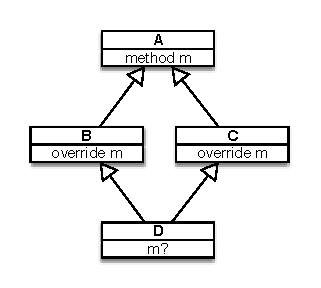
\includegraphics{figures/diamond.eps}
    \subcaption{The diamond problem} \label{fig:diamond}
  \end{subfigure} ~
  \begin{subfigure}[b]{0.45\textwidth}
    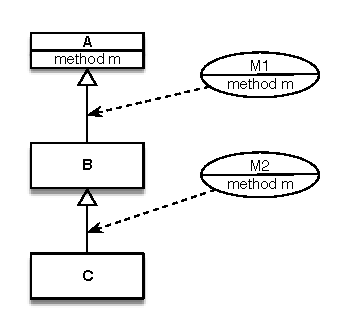
\includegraphics{figures/mixin.eps}
    \subcaption{Mixin composition} \label{fig:mixin}
  \end{subfigure}
  \caption{Multiple inheritance and mixins}
\end{figure}


Mixins and traits are two well-studied mechanisms to provide some form of
multiple inheritance. Mixins~\citep{bracha1990mixin} provide a simple mechanism
for multiple inheritance without the ambiguity issue. A mixin is a subclass
declaration parameterized over a superclass. Or simply put, a mixin can be
treated as a function from classes to classes. Thus the same mixin can be used to
extend a variety of parent classes with the same set of features.
\Cref{fig:mixin} shows a typical class hierarchy when using mixins. In the mixin
model, a class can inherit from another class by means of single inheritance as
usual. Apart from that, it can also have several mixins applied \textit{one at a
  time}. Let us take a close look at \cref{fig:mixin}. Both mixins
\lstinline{M1} and \lstinline{M2} contain a method \lstinline{m}, a question
arises as to which one is inherited in the class \lstinline{C}. The answer is
\lstinline{m} from the mixin \lstinline{M2}. This is because mixin composition
is \textit{linear}: methods defined in mixins appearing later override all the
identically named methods of earlier mixins. While this simple mechanism does
avoid conflicts, it also lead to other problems. For example, though we can
obtain the method \lstinline{m} from the mixin \lstinline{M1} by switching the
order of \lstinline{M1} and \lstinline{M2}, no suitable order of composition
exists to obtain \lstinline{m} from the superclass \lstinline{A}.

In respondence to the problems in the then compositional models,
\citet{scharli2003traits} proposed a mechanism called \textit{traits} as a
better way to foster code reuse in object-oriented programs. A trait is
essentially \textit{a set of pure methods}, divorced from any class hierarchy. A
trait \textit{provides} a set of methods to implement the behavior, and it may
also specify a set of \textit{required methods} that parameterize the provided
behavior. \Cref{fig:trait} shows a simple trait \lstinline{TCircle}, which
provides two methods \lstinline{hash} and \lstinline{area}, and requires a
method \lstinline{radius}. A class is then constructed by inheriting from a
superclass and incorporating a collection of traits, as shown in
\cref{fig:trait:conflict}. Also notice that there is a conflicting method
\lstinline{hash} that is provided by both \lstinline{TCircle} and
\lstinline{TDraw}. This is where the trait model is very different from the
mixin model. Unlike mixins that force a linear order in their composition,
traits can be composed in arbitrary order, and as a consequence, conflicting
methods must be resolved \textit{explicitly}, either by overriding the
conflicting methods, or by excluding a method from all but one trait.
\citet{scharli2003traits} discuss several other issues with mixins, which can be
improved by traits. We refer to their paper for a detailed account of traits.


\begin{figure}
  \centering
  \begin{subfigure}[b]{0.45\textwidth}
    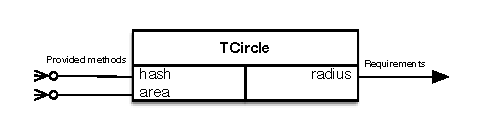
\includegraphics[scale=0.85]{figures/trait1.eps}
    \subcaption{A simple trait} \label{fig:trait}
  \end{subfigure} ~
  \begin{subfigure}[b]{0.45\textwidth}
    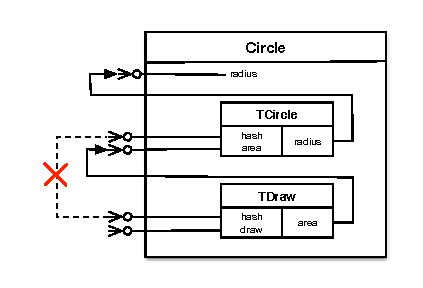
\includegraphics{figures/trait3.eps}
    \subcaption{Trait composition with conflicts} \label{fig:trait:conflict}
  \end{subfigure}
  \caption{Traits and conflicts}
\end{figure}

%%% Local Variables:
%%% mode: latex
%%% TeX-master: "../Thesis"
%%% org-ref-default-bibliography: ../Thesis.bib
%%% End:
